\documentclass[a4paper,10pt]{article}
\usepackage[utf8x]{inputenc}

\usepackage{times}

\usepackage[pdftex]{graphicx}
\usepackage{epstopdf}
\usepackage{subfig}
\usepackage{float}

\usepackage[english]{babel}

\usepackage{anysize}
\marginsize{2cm}{2cm}{1.5cm}{2cm}

\usepackage{tabularx}
\usepackage{amsmath, amssymb, latexsym}
\usepackage[colorlinks=true, urlcolor=blue, citecolor=red]{hyperref}
\usepackage{datetime}


\newcommand{\titulo}[2]{ \begin{titlepage}\begin{center}\vspace*{\fill}\textsc{\Huge #1}\\[3cm]  
\includegraphics[scale=0.3]{./zlogo.png} \\[3cm]\emph{Realized by:}\\ \textsc{Jacinto Arias Martínez}\\ \textsc{Adrián Sánchez López}\vspace*{\fill}\vfill\monthname[\the\month],\, \the\year\end{center}\end{titlepage}}

\newcommand{\p}[1]{\paragraph{\indent\textnormal{#1}}}



\begin{document}

 \titulo{ARTIFICIAL INTELLIGENCE IN VIDEOGAMES}{Practice project}

    \begin{abstract}
    
    \end{abstract}

  \newpage

  \vspace*{3cm}
  \tableofcontents
  \vspace*{\fill}

\newpage
\section{Project definition and design principles}

  \subsection{Game definition}

    \p{The game we are proposing is an \textbf{RTS} game in which you will be managing a large horde of units in order to break down a enemy fortress.}

    \p{The main feature of this game is that you won't be able to directly control your units, in case of that, you will give them orders and the units should behave according to them but with a high free will grade.}

    \p{The horde will be separated into groups of units that you will be able to select. Using the mouse and the graphic interface provided, you will be able to control a group of unit at once, giving orders to your troops should alter its behaviour and they will follow your order in their way.}

    \p{There will be computer controlled enemies that will kill your units in order to defeat you. A longer description will be included in the next section.}


  \subsection{Motivation}

    \p{We have chosen this kind of game because we think that the AI integration possibilities are huge. AI principles can be integrated in many of the game components, for example, in the game engine, AI techniques can be used in order to define and implement the units free will, also it can be combined with an agent-based approach. AI could also be applied to make opponents for the game, we should define their strategies, decision, etc...}


  \subsection{Game classification}

    \p{The presented game could be classified as:}

    \begin{itemize}
     \item \textbf{Game type:} Real Time Strategy
     \item \textbf{Type of use:} The machine is controlling several characteristics as physics, ground generation and playing as an opponent.
     \item \textbf{Theme:} Horde of units.
     \item \textbf{User age:} No children are allowed to play this game because of the violence it contains.
     \item \textbf{Skills development:} In this game player will develop spatial abilities and also reasoning ones by controlling the units and thinking fast strategies in order to win the game.
     \item \textbf{Platform:} Originally it is developed for PC, with compatibility with Microsoft Windows and Linux.
     \item \textbf{Technology development:} All the game has been developed using free software: Ogre 3D, Blender, Gimp, OIS and OpenAl.
     \item \textbf{Development company:} Jacinto and Adrián or Adrian and Jacinto Developing.
     \item \textbf{Year of development:} 2012.
    \end{itemize}

    

\newpage
\section{Artificial intelligence principles I: Computational Theory}

  \subsection{Game elements}

    \p{In this game your goal is to conquer the centre of the map by getting a large number of zombies inside the enemy fortress.}

    \p{There are four main elements on the game:}

    \begin{itemize}
     \item \textbf{Zombies:} This is the interactive element of the game. You will control a few groups of zombies that will start spread over the map. You can order to each group of zombies move to a point, but if they are hungry they won't obey you and will wander randomly. If they can reach \textit{the goal} (centre of the map) they should attack the enemy, but beware because they can shoot and kill the zombies.
  
	\begin{figure}[hbt]
	    \begin{center}
		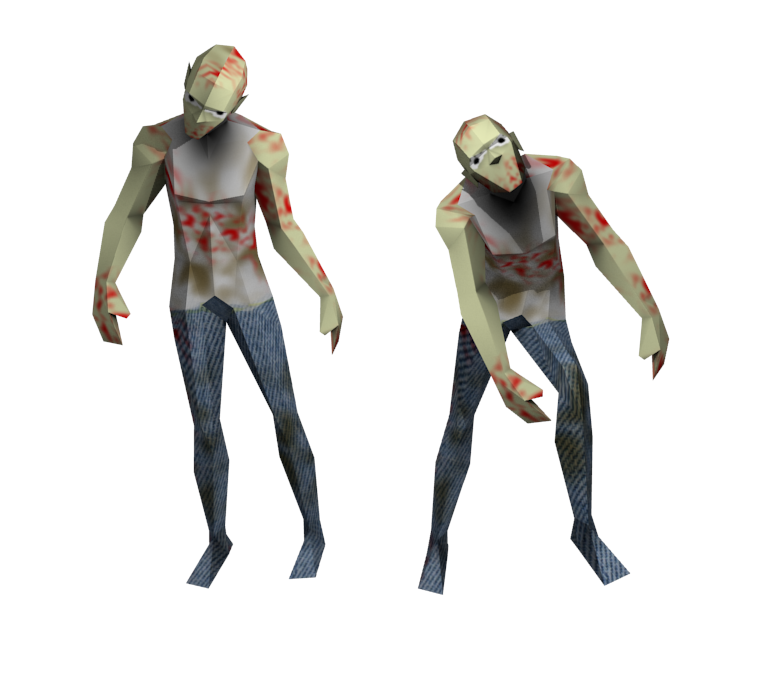
\includegraphics[scale=.8]{zombies.png}
	    \end{center}
	    \caption{Zombie models.}
	    \label{fig:rb1}
	\end{figure}

     \item \textbf{Food:} Spread along the map you can also find food, food is necessary for the zombies to get strong and obey your orders. If a group of zombies find food they will eat it.

      \newpage
     \item \textbf{Enemies:} In the centre of the map, and spread along it, you will find a bunch of enemies. They will be patrolling all the time and trying to kill your zombies if they come close enough. Your goal is to kill every enemy on the map (or reach the goal).
  
	\begin{figure}[hbt]
	    \begin{center}
		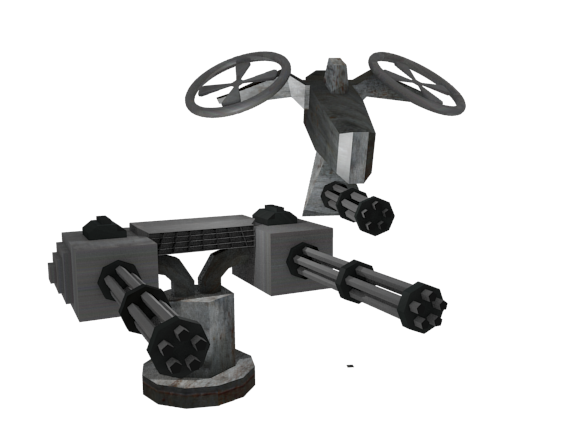
\includegraphics[scale=.8]{enemies.png}
	    \end{center}
	    \caption{Enemy models.}
	    \label{fig:rb2}
	\end{figure}

     \item \textbf{Goal:} The goal of the game is to catch the centre goal, a \textit{big Brain}. If a zombie touch the Brain, you will win; but is not too easy because all the enemies are patrolling and protecting the goal.

	\begin{figure}[hbt]
	    \begin{center}
		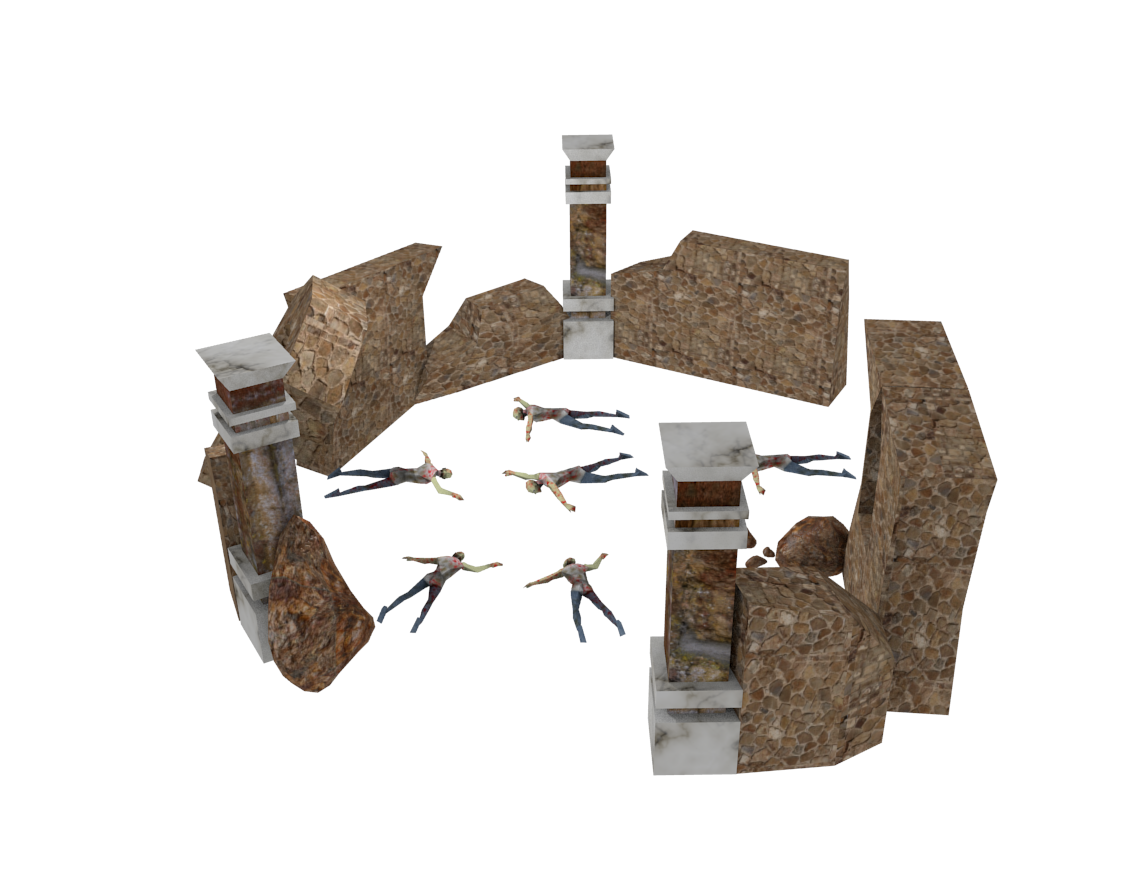
\includegraphics[scale=.6]{goal.png}
	    \end{center}
	    \caption{Goal model.}
	    \label{fig:rb3}
	\end{figure}

    \end{itemize}

  \p{You can also find obstacles and other passive elements along the map, such as plants, trees, rocks \dots. That will make your zombies harder to move in a pack.}

\newpage
  \subsection{Knowledge extraction}

    \p{The basic strategy a user has to know about how to play this game is that everything has to be accomplished by using a large number of units. Some enemies would be tougher than others so you should take a look of the map before start to send all your units to an early end.}

    \p{When you plan your attack watch for fixed turrets or enemies in far positions in order to avoid them and don't waste troops killing them. Also, coordinate your units to attack at once and corner the stronger enemies to quickly take them down before they cause so many casualties.}

    \p{The food should be a secondary goal, but you should collect many of them in order to make your army stronger for the last assault if you want your plan to be committed. Otherwise, your troops will fall into chaos and wander around the map letting the enemies to slowly kill them.}

    \p{The game is simple, so when you discover how the different enemies behave you should be able to anticipate you plan by taken a quick look of the map disposal.}

  \subsection{Artificial intelligence applications}

  \p{In this section we will identify some of the problems that can be solved using artificial intelligence solutions.}

  \p{The most immediate problem to solve is the behaviour of the units. With most of the techniques we should solve problems like \textit{units movemen}t, \textit{path finding}, \textit{collision avoidance} or \textit{unit tracking}.}

  \p{Other aspect of the game that can be involved in AI developing can be the opponent strategy. We can implements such methods in order to give the opponent more intelligence making the game most interesting. For example we can apply these techniques for choosing the army or placing in on the map.}

  \subsubsection{Movement problems}
    
    \p{When speaking about movement we have to difference between zombies and enemies, because their movement models are not the same.}

    \p{The zombies model is based in two parameters, firs of all we have the destination point which is the zombies goal to reach, on the other hand we have the hunger of the zombies group. If the zombies \textit{are hungry} they would tend to \textit{wander around} while reaching the point, if the hunger level gets low the zombies will appear to come closer to the point obeying the player's order directly.}

    \p{When programming the zombies movement we should take those parameters in consideration and apply an straight movement and a movement pattern for randomness when wandering. These movement pattern should be applied by using AI techniques, with different techniques we could achieve richer patterns going from a random pattern to behaviours like \textbf{birds flocks}, \textbf{particle swarm} or something different.}

    \p{A \textit{rules based system}, a \textit{neural network} or \textit{CBR} can be implemented to achieve this.}

   \subsubsection{Path finding and collision avoidance}

    \p{This problem is mostly a feature of the game engine. With the integration of a physics module which will simulate the collisions of solid models there should be physical interaction between the elements of the game. For example, a unit will not be able to pass through a tree or a wall or also through another unit; also, it will have to adapt its movement to the terrain topology.}

    \p{For that reason, when a element is commanded to move through the map the game engine should find for him a valid path in order to keep the movement realistic and avoiding that element (normally and avatar) to get stuck in somewhere.}

    \p{Normally, those path finding problems can be solved applying heuristic search techniques like the A star algorithm.}

   \subsubsection{Opponent strategy}

    \p{At first, the game is being designed as a single player one. For that reason an AI should be designed and programmed in order to control the opponent.}

    \p{This AI system should variate in complexity, different models and behaviours can be programmed in order to give the game a different approach. For example, a simple rule based system can be implemented in order to do that conferring the an ``arcade'' approach. However, we can also integrate an combination of different AI techniques even including learning, to make a robust opponent for a different kind of game with also a really good academic interest.}

    \p{Independently of the selected system, the problems that should be solved by it are the same:}

    \begin{itemize}
     \item \textbf{Moving} and \textbf{positioning} the units.
     \item \textbf{Look for}, \textbf{select} and \textbf{attack enemies}.
    \end{itemize}
  
    \p{Those problems can be solved using a very simple system or using a high-level complicated strategy.}

    \p{To commit this task, we provide a framework in order to identify a limited number of elements to work with:}

    \begin{itemize}
     \item \textbf{Enemy behaviour:} There are two behaviours in which the enemy can be at a given moment:
	 \begin{itemize}
	    \item \textit{Patrol}: The enemy is moving around the map, moving to a given point that the punctual movement provider tells it.
	    \item \textit{Seek}: The enemy is rotating over himself at a constant speed, can be done for searching enemies in range.
	  \end{itemize}

     \item \textbf{Enemy aggressiveness:} The enemy can be in an aggressive mood or not. If aggressiveness is on, the enemy would shoot at anything that comes into range.
     \item \textbf{Environment data:} The enemy can know at any moment about its own data and the zombies data over the map with no restriction.
    \end{itemize}

    \p{Additionally to those elements, each unit has different parameters, that would make it stronger o weaker:}

      \begin{itemize}
       \item \textbf{DPS: Damage Per Second:} Is the amount of damage that an enemy deal to the zombies.
       \item \textbf{Life:} The amount of damage that an enemy can be dealt by zombies before die.
       \item \textbf{Range:} The maximum distance that a unit cat attack.
       \item \textbf{Speed:} The velocity of the enemy displacements around the map.
      \end{itemize}

    \p{Using all of these elements we should implement all of the different AI for the different kind of enemies in the game. In further sections we will explain about the different implementations.}



  \newpage
\section{Artificial intelligence principles II: Representation and algorithms}

  \subsection{Application of search techniques}

    \subsubsection{Path finding}
    \p{As we said above, we can apply those techniques in order to find correct paths for the units to move. In order to solve the problem we will use the popular A star algorithm, and for that we have defined the next representation scheme:}

    \begin{itemize}
     \item \textbf{Input space:} As an input the algorithm will receive the game's map divided in regions and represented as a non directed graph where each node will be either a passable or an impassable region, the actual location of the unit to move and the final location where the unit want to reach. The arcs of the graph will be weighted with the distance between regions and only the nodes which represents adjacent region will be connected.
     \item \textbf{Output space:} As an output the algorithm will return a valid path of the graph, directly interpretable by the game engine.
     \item \textbf{States:} An stated will be conformed by a node on the graph. Only the nodes that are passable can be considered as valid states. 
     \item \textbf{Initial state – Final state:} The initial state corresponds to the node which represents the region of the map where the unit is located. The final state is the one conformed by the desired location.
     \item \textbf{Operators:} Ramification through states should be done by moving directly to the neighbours of the current node.
     \item \textbf{Function of heuristic evaluation:} The heuristic function will just be the cost of the path of going directly from the origin to the destination without considering the condition of the regions. The distances will be precalculated for the algorithm.
    \end{itemize}

  \subsection{Application of rule based systems}
  
    \subsubsection{Movement model: Simulation of a birds flock}

      \p{As we said, we can use a RBS in order to provide a model of movement for our units. In this case it will be a simple one with a really small set of rules but when applied to a group of units it is fully functional and provides emergent behaviours so this could also be seen as an \textbf{artificial life} system.}

      \p{For the implementation which will be explained later we have defined the next representation scheme:}

      \begin{itemize}
      \item \textbf{Input space:} As an input space we provide as antecedents the unit actual location, and the other units actual location.
      \item \textbf{Output space:} As an output space the system returns a destination location where the unit will go as the movement module expect.
      \item \textbf{Input and output representation:} The locations are represented as 2D points in a cartesian system, so we can make some calculations on them.
      \item \textbf{Statements base:} Nearest unit distance.
      \item \textbf{Set of rules (knowledge injected):} The set of rules consists of three of them, enough to provide an approximation for the \textbf{birds flock behaviour}. The rules are the following, ordered by highest priority:
	  \begin{itemize}
	    \item \textit{If you are far away from other birds, head toward the nearest bird.}
	    \item \textit{If you are about to crash into another bird, turn around.}
	    \item \textit{Otherwise, fly in the same direction as the bird next to you.}

	  \end{itemize}
      \item \textbf{Considerations for the inference engine:} As this will be a really short inference cycle, the inference engine will be emulated using sequential conditional and the statement base using numerical variables.
      \item \textbf{¿Learning?:} As this system is based on purely injected knowledge it will be difficult to include any learning. Perhaps the distance parameters of that appears on the rules should be later optimized.
      \end{itemize}

	\begin{figure}[hbt]
	    \begin{center}
		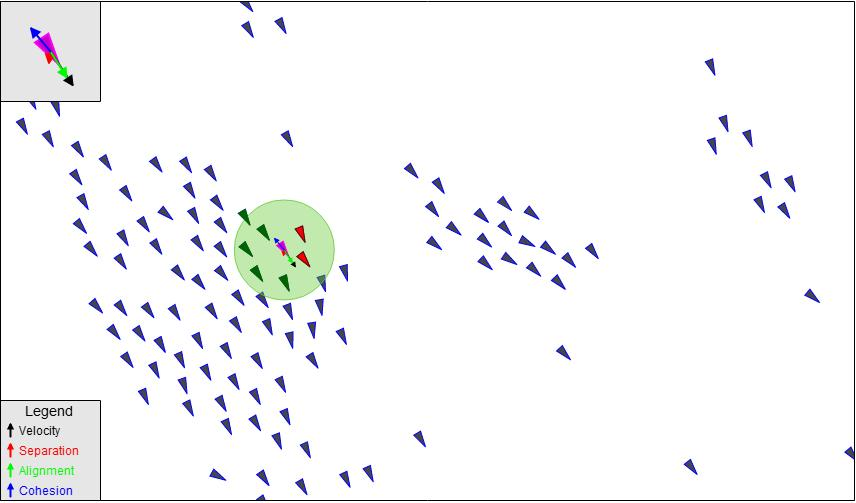
\includegraphics[scale=.7]{flocking.jpg}
	    \end{center}
	    \caption{Birds flock behaviour.}
	    \label{fig:rb4}
	\end{figure}

    \subsubsection{AI behaviour: The hunter}

      \p{By using a simple set of rules, we can make a very effective opponent using a really low resources consuming technique.}

      \p{For the implementation which will be explained later we have defined the next representation scheme:}

      \begin{itemize}
      \item \textbf{Input space:} As an input space we provide as antecedents the unit actual location, and the zombies locations.
      \item \textbf{Output space:} As an output space the system returns the next action to achieve, that could be move to a given point or to stay and seek for enemies.
      \item \textbf{Input and output representation:} The locations are represented as 2D points in a cartesian system, so we can make some calculations on them, the output is given directly to the program to interpret it.
      \item \textbf{Statements base:} Previously attacked unit, nearest unit location.
      \item \textbf{Set of rules (knowledge injected):}
	  \begin{itemize}
	    \item \textit{If the nearer enemy is too close move away before attacking it.}
	    \item \textit{If an enemy gets in range, shoot at it.}
	    \item \textit{If you has just killed and enemy, stay and seek for the rest of the pack}
	    \item \textit{If you don't have an objetive move closer to the nearer enemy.}

	  \end{itemize}
      \item \textbf{Considerations for the inference engine:} As this will be a really short inference cycle, the inference engine will be emulated using sequential conditional and the statement base using numerical variables.
      \item \textbf{¿Learning?:} As this system is based on purely injected knowledge it will be difficult to include any learning. Perhaps the distance parameters of that appears on the rules should be later optimized.
      \end{itemize}


\subsection{Not implemented techniques}

    \p{The next techniques don't have a formalized representation scheme for our game, but they have been discussed and proposed for typical usages inside this game.}

    \p{The information provided next consists in factional ideas that could be revised and implemented in a more mature stage of development of our game. By the moment, we provide this information as an exercise for the current subject.}

  \subsubsection{Application of CBR}

    \p{The idea is to use CBR in order to define some strategies for the opponent, giving more flexibility than a RBS. We have different strategies for the opponent, and we need to choose one.
	The possible strategies are: \textbf{patrol}, \textbf{explore}, \textbf{attack to zombie detected} or \textbf{protect the Brain}.}

    \p{The Case-based reasoning has been formalized as the following a four-step processes:}

      \begin{itemize}
	\item \textbf{Select:} Given a target problem, retrieve from memory cases relevant to solving it. A case consists of a problem, its solution, and, typically, annotations about how the solution was derived. 

	For our problem of select the correct strategy, we retrieve from our database the most case relevant (with best solution) that solve the choice with the actual status.

	\item \textbf{Matching} Map the solution from the previous case to the target problem. This may involve adapting the solution as needed to fit the new situation.

	Adapt the retrieve solution to include all the particularities of actual situation, such as different number of zombies, positions, and so on.

	\item \textbf{Review} Having mapped the previous solution to the target situation, test the new solution and, if necessary, revise. 

	We need to check, if after adapt the retrieve solution of strategy selection, this is a valid solution to the problem or we can not solve the choice. If a solution do not give good results (is not valid ), we need to make a revision, such as modify the selection trying to do a better solution.

	\item \textbf{Update} After the solution has been successfully adapted to the target problem, store the resulting experience as a new case in memory.

	When we have a new successfull selection of a strategy, we include it to out database like a new case for future steps.

      \end{itemize}

    \p{The point of using this kind of techniques is that we can but it in the game and face it against human players to see how it evolves.}

     \p{A good variation of this should be using it to adjust the selected strategies of each enemy in the map. It could be used as a \textbf{meta-algorithm} to do that, designing and initial configuration of the AI system by assigning a pre-made behavior to each unit and evaluating the result at the end of the game.}

  \subsubsection{Application of connectionism}

      \p{The idea of connectionism is really similar to the previous one.}

      \p{By using the different states of the enemies, and the enviromental information we can design a multi-layer neural network which outputs would be the next behaviour that the enemy should get to practice.}

      \p{The big problem with this kind of model is the need of learning. With the \textbf{CBR approach} we would be able to put it in the game and teach it by playing with human players, but the \textbf{neural network} learning process is \textbf{more complex} and requires more simulation that would be really \textbf{difficult to make} without the intervention of an human player.}

  \subsubsection{Evolutionary computation}

  
  \subsection{Mathematical approaches and other algorithms}

    \p{As this game is a simple one, most of evaluated problems can be and have been solved by using more simple solution than using complex AI techniques.}

    \p{Basic algorithms, and mathematical approaches have been applied in some situations that we are going to explain next.}

    \subsubsection{Collision system and geometry navigation}

      \p{For physics, like collisions, we've implemented mathematical solution based on raytracing. Those solutions are based in linear algebra and analitic geometry. So mathematical equations had been implemented directly in the code in order to solve the problem of collisions or for example, calculating the range of fire for the enemies weapons.}

      \p{Also mathematical equations have been implemented in order to manage the navigation through the map. Elemental trigonometry and analitic geometry has been used in order to provide the mathematical support to spatial navigation.}

    \subsubsection{Randomness}

      \p{Randomness is deeply used in this game. For a lot of situations a random number is able to solve a problem and also to add some richer properties to the game, making it more stochastic and so amusing for the players.}

    \subsubsection{Directly applied knowledge}

      \p{In some situations, it could be a good point to directly apply some of the knowledge extracted directly by using simple programming techniques.}

      \p{Although we could try to formalize some of this implementations by using some of the previous techniques, most of them are too simple for that. So state machines, search algorithms and other basic programming techniques can be found deeply used in some of the AI modules and can be considered as cornerstones.}

  \subsection{Cooperative behaviour}

      \p{Cooperative behaviour should be a good point to add to this game.}
      
      \p{We just have to add the other enemies information to the environmental information they get and use it properly. We have two ways of doing this:}

	\begin{itemize}
	 \item \textbf{Define a communication protocol:} By establishing a direct communication between the enemies they could use joint strategies in order to win the match to the player. Movement formations or spread themselves along the map to cover more area.
	 \item \textbf{Define an overlord controller:} This kind of controller could make more meta-game level strategies like a human player. And so the extracted knowledge could be applied here.
	\end{itemize}

      \p{Despite of the selected technique, cooperative behaviour an agent based approach would enhance the emergent behaviours of the units in the game, giving it a more ``intelligence'' appearance.}

\newpage
\section{Artificial intelligence principles III: Implementation}

  \subsection{Software engineering and game engine implementation issues}

    \p{As this subject is not focused on videogames programming, this section will cover the basis of the implementation in order to identify and follow the different elements of the game engine. We are going the provide the fewer diagrams and models needed to understand the structure and the function of this application.}

%%
%%	SI NO SE PONE NADA MAS NEJOR BORRAR DIGO YO.

  \subsection{Programing with Ogre3D}

    \p{\textbf{OGRE} (\textit{Object-Oriented Graphics Rendering Engine}) is a scene-oriented, flexible 3D rendering engine (as opposed to a game engine) written in \textbf{C++} designed to make it easier and intuitive for developers to produce applications utilizing hardware-accelerated 3D graphics. The class library abstracts the details of using the underlying system libraries like \textit{Direct3D} and \textit{OpenGL} and provides an interface based on world objects and other high level classes.}

    \p{The learning curve of OGRE is very high, it costs a lot to adapt and understand all the systems and methods for developing a first application.}

    \p{But on the other hand, once you have come to understand its operation, continue to develop and incorporate new functionality is much more fluid. But how OGRE is only a rendering engine, we need other kind of software to desing our models and animation. We have choose Blender for 3D modeling.}

	\begin{figure}[hbt]
	    \begin{center}
		
\includegraphics[scale=.4]{ogrelogo.jpg}
	    \end{center}
	    \caption{Logo of Ogre 3D.}
	\end{figure}

  \subsection{Artwork in Blender and Gimp}

    \p{\textbf{Blender} is a free and open-source 3D computer graphics software product used for creating animated films, visual effects, interactive 3D applications or video games. Blender's features include 3D modeling, UV unwrapping, texturing, rigging and skinning, fluid and smoke simulation, particle simulation, animating, rendering, video editing and compositing. It also features a built-in game engine.}

    \p{\textbf{GIMP} (GNU Image Manipulation Program) is a free and open source software image retouching and editing tool. Gimp has tools used for image retouching and editing, free-form drawing, resizing, cropping, photo-montages (combining multiple images), converting between different image formats, and more specialised tasks. }

  \begin{figure}[hbt]
      \centering
      \subfloat[Logo of Blender]{\label{fig:cima}
\includegraphics[scale=.35]{Blender-Logo.jpg}} \qquad
      \subfloat[Logo of Gimp]{\label{fig:cimb}
\includegraphics[scale=.35]{GIMP-logo.png}}
      \caption{Blender and Gimp Logos.}
      \label{fig:res}
   \end{figure}

    \p{As Blender is just a 3D modeling software, our models and animations need to be exported to use it on OGRE aplication. First of all, we desing the 3D geometry of, for example, a zombie in Blender; then, include some textures and details with an external 2D editing software (like GIMP), and finally export our model to a OGRE format.}


  \subsection{AI techniques integration}

  \p{In this section we will talk about the structure of the game engine and how we should integrate the different techniques in order to provide not only a videogame but also a modular platform in which we can test the different approaches seen in class and study its behaviours.}

  \p{On the one hand and as the game engine, we are going to introduce the different elements that we should integrate to provide a videogame interface and its elements. On the other hand as a platform for testing AI techniques we are going to let an empty place in which we can plug in the AI techniques as different modules implementing an specific model; for example, we are going to implement the hordes units movement in the game engine letting a place to plug in a model, which can be a random model or a richer approach like a rule based system or a neural network.}
  
  \subsubsection{Movement module and models}
    
    \p{The movement models for the units will affect to their free will movements during the game. Providing richer model will make the make more interesting as our avatar should behave in a more complex way and also resulting on situations of emergency.}

% NO PUEDO INSERTAR UN EPS (sera porque me faltan esas librerias, nose)
% 	\begin{figure}[hbt]
% 	    \begin{center}
% 		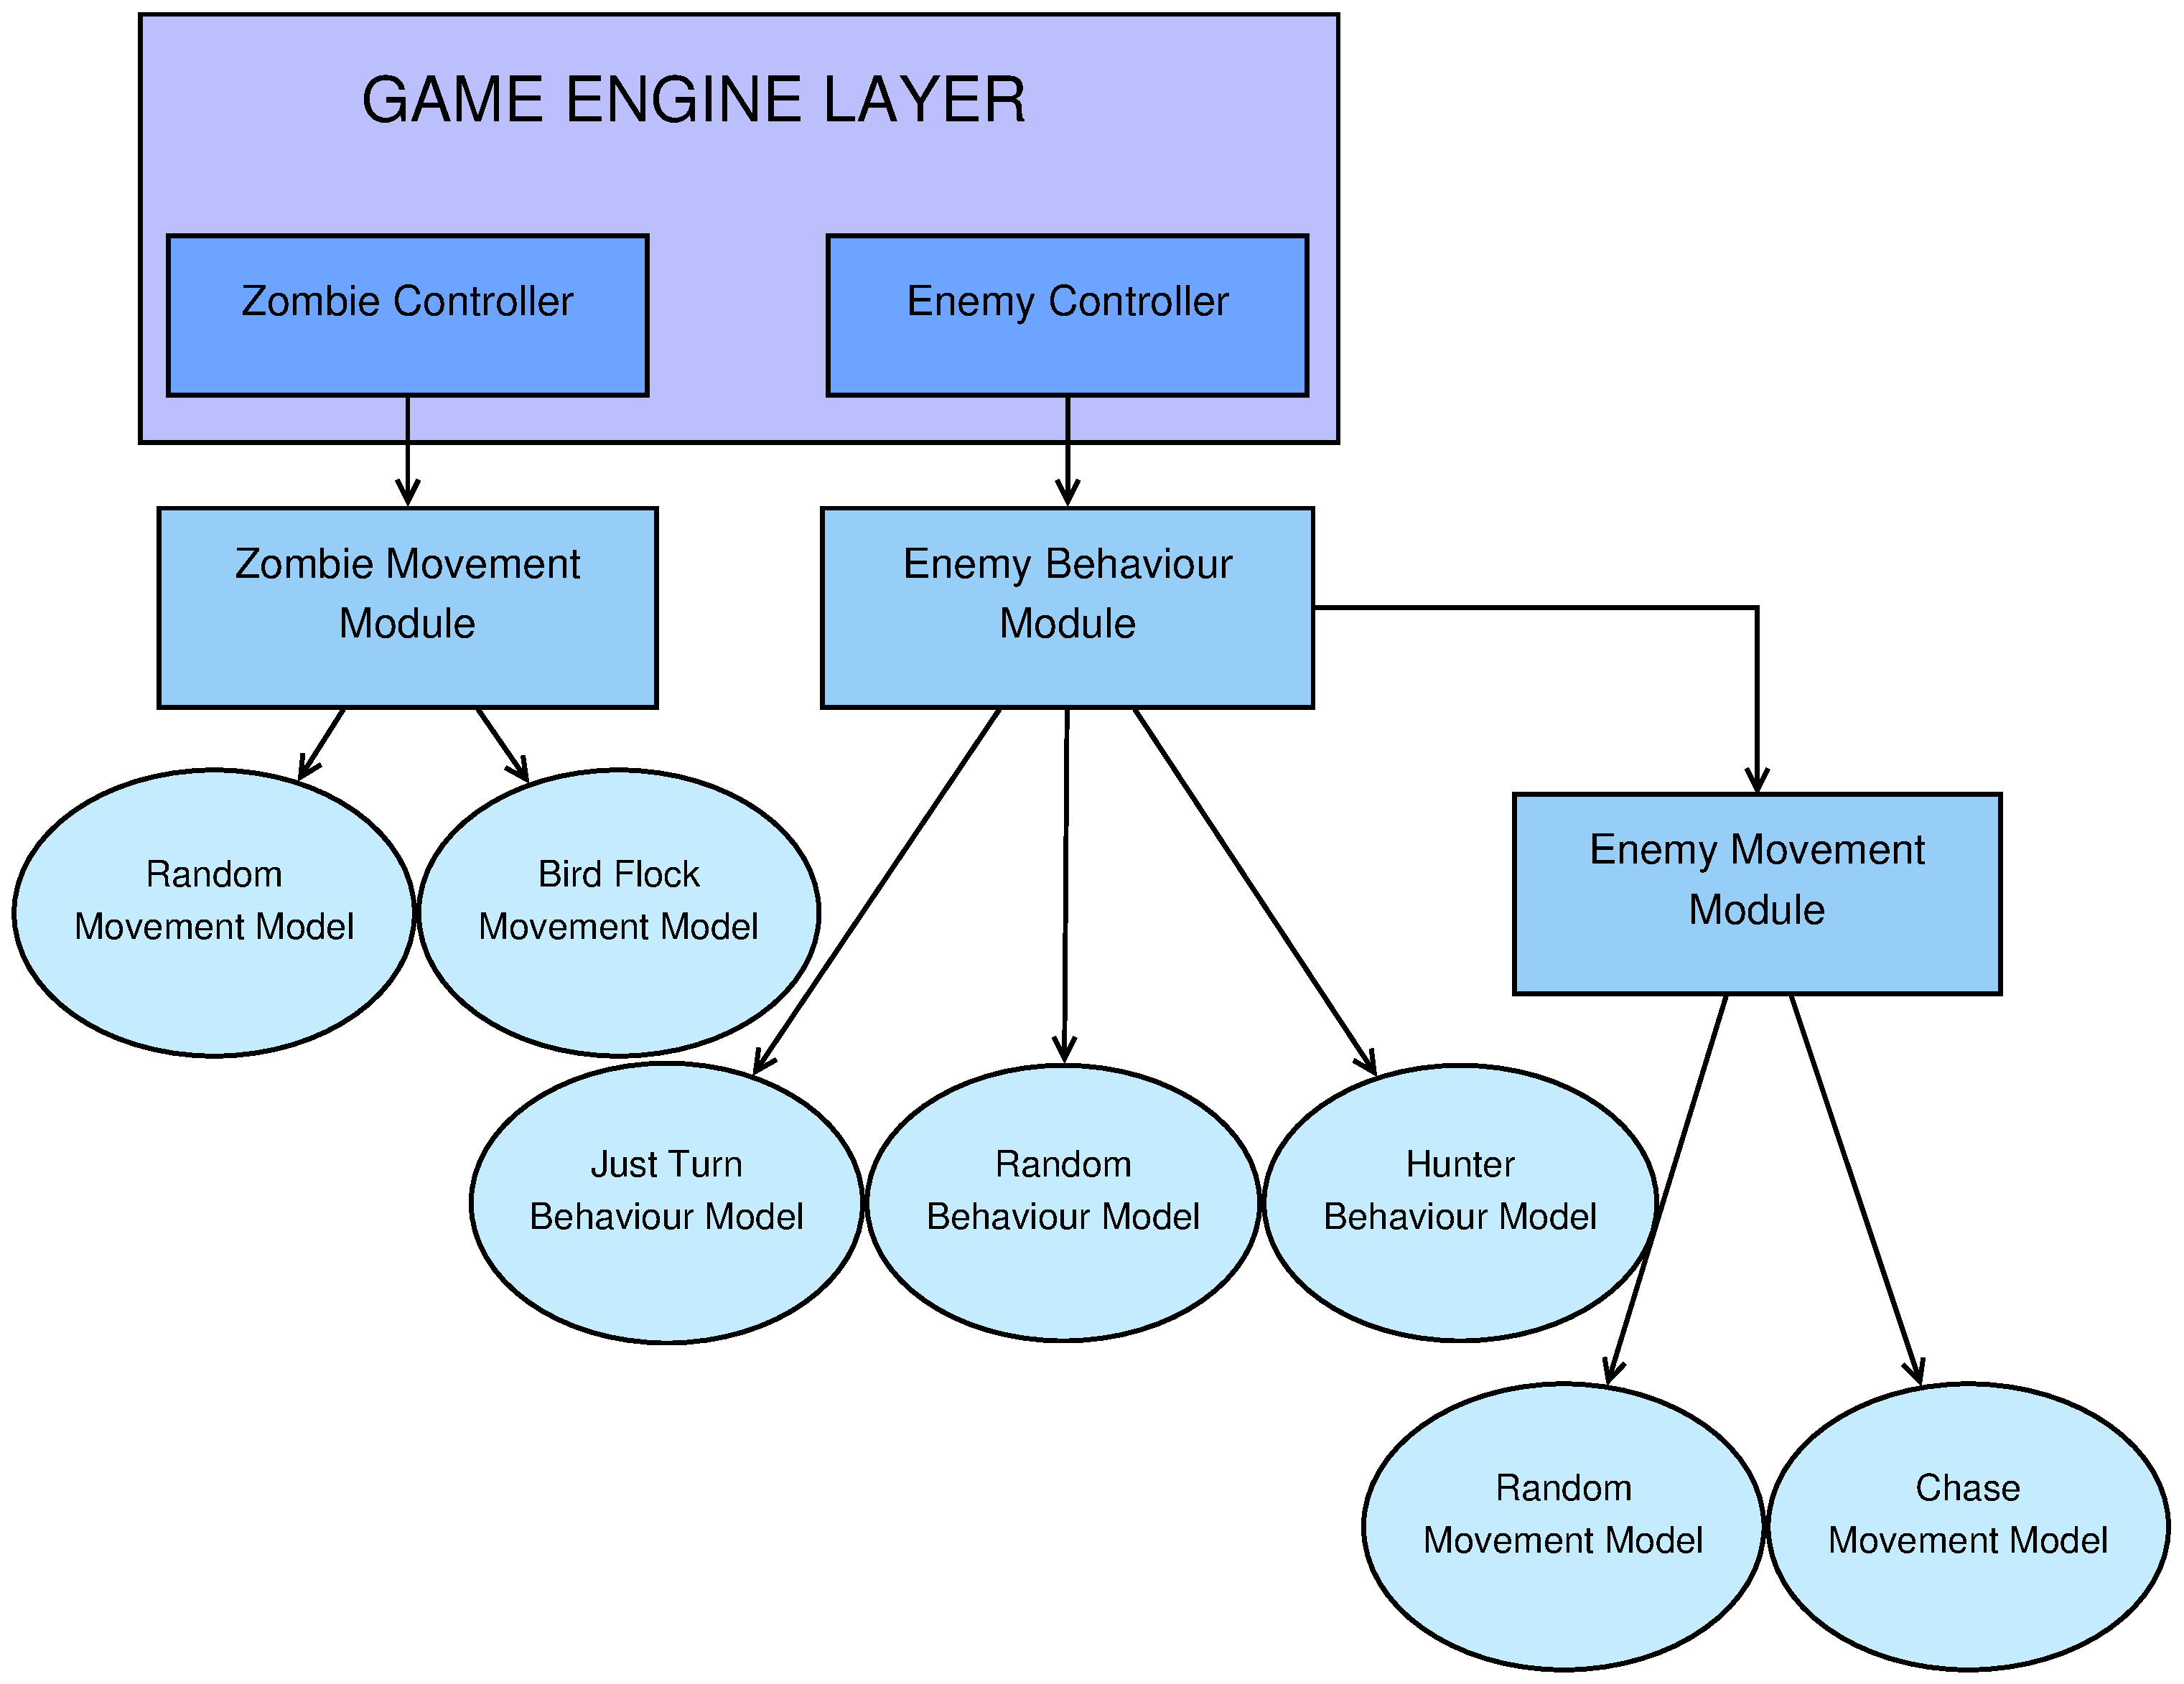
\includegraphics[scale=.4]{modulos.eps}
% 
% 	    \end{center}
% 	    \caption{Movement and Behaviour modules.}
% 	\end{figure}

    \p{The movement module itself should catch some of the parameters from the units and environment and provide a function \textit{calculateMove()} that, for a given avatar, will calculate the next move.}

    \p{The next models have been included in the game and all fully interchangeable without changing anything on the code rather than its name:}

    \begin{itemize}
     \item \textbf{Random model:} As it name says it model should give a random movement to each unit that ask for it. Normally units following this model would move on any direction without taking care of anything else (environment or other units).
     \item \textbf{Bird Flock:} This model is based on a biological approach and has been implemented by using a ruled based system, the specification is shown before in its own section. With this model the whole group will maintain some coherence and will move along together, it neither has any consideration on the environment.
    \end{itemize}


  \subsubsection{Behaving and action module and models}

  \subsubsection{Strategy and meta-game module and models}


\section{Conclusions}

  \subsection{AI Results}
    \p{We have obtained the following results, in terms of artificial intelligence behavior:}
    TO DO

  \subsection{Development costs}
    \p{The approximate time invested in the development of the application has been:}
    TO DO

  \subsection{Showing}
    \p{Some samples screenshots of the application Zproyect:}

	\begin{figure}[hbt]

	\p{ A possible initial situation of enemies, protecting the goal. \newline}
  
	    \begin{center}
			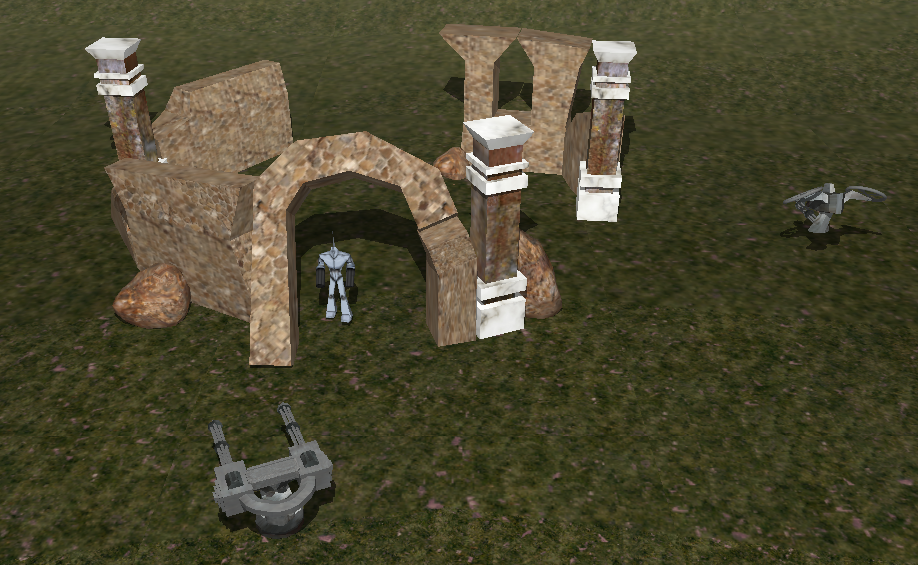
\includegraphics[scale=.5]{captura1.png}
	    \end{center}
	    \caption{Gameplay screenshot of enemies and goal.}

	\end{figure}

	\begin{figure}[hbt]	
	\p{When enemy robot can see zombies in his range, does not doubt, he only attack. \newline}
    
	    \begin{center}
			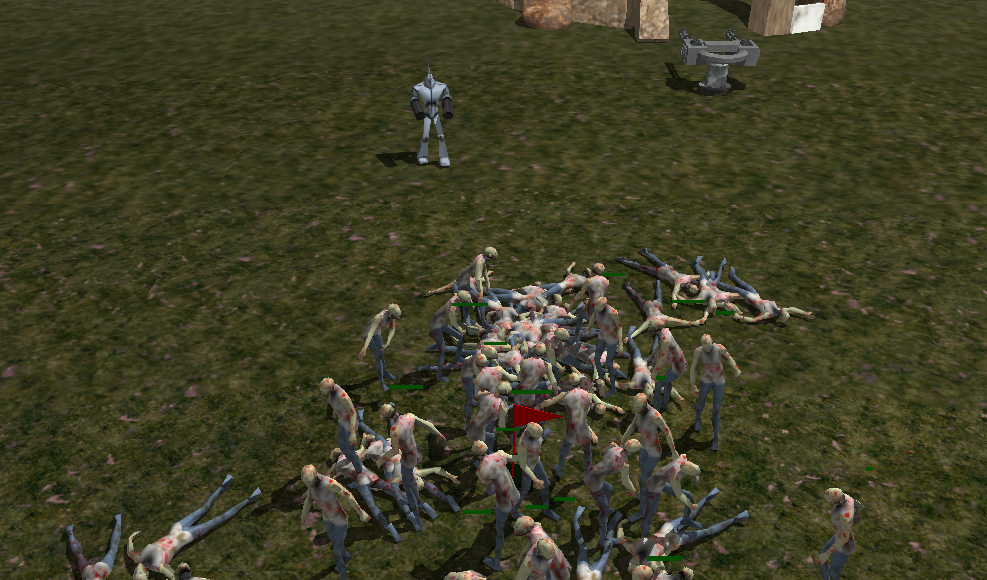
\includegraphics[scale=.6]{captura2.png}
	    \end{center}
	    \caption{Zombies killed by a robot.}
	\end{figure}

	\begin{figure}[hbt]
	
	\p{But if the zombies reach to a enemy, they can kill it too. \newline}    
	    \begin{center}
			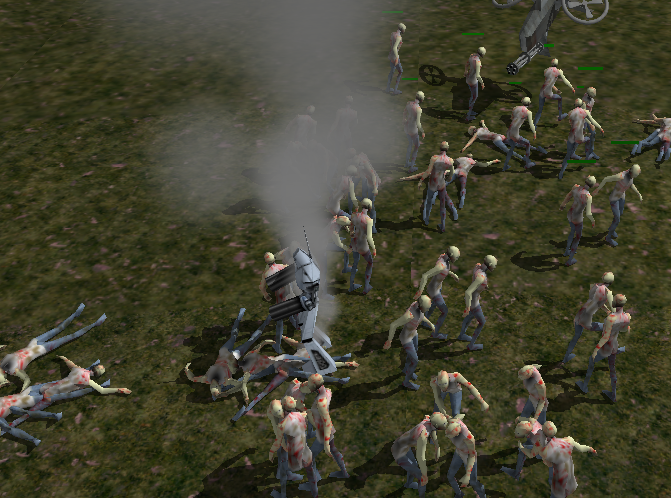
\includegraphics[scale=.7]{captura3.png}
	    \end{center}
	    \caption{Enemy robot killed by zombies.}
	\end{figure}


	\begin{figure}[hbt]	
	\p{And is easier to kill a turret. \newline}    
	    \begin{center}
			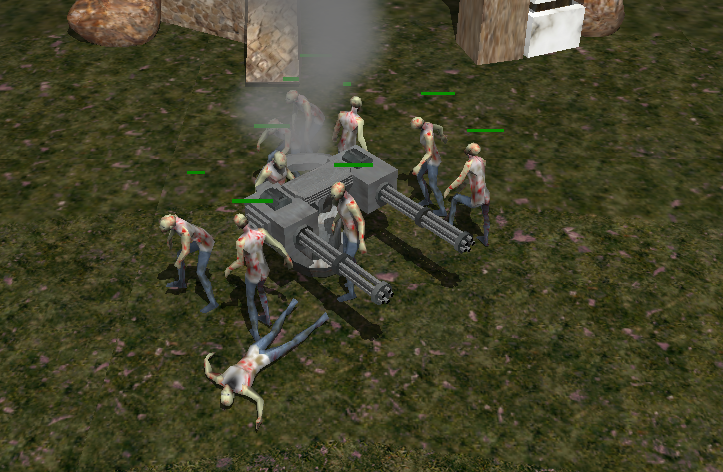
\includegraphics[scale=.7]{captura4.png}
	    \end{center}
	    \caption{Enemy turret killed by zombies.}
	\end{figure}

	\begin{figure}[hbt]	
	\p{The ideal way to play, would be more than \textbf{five hundred} zombies, wandering the world. \newline}
    
	    \begin{center}
			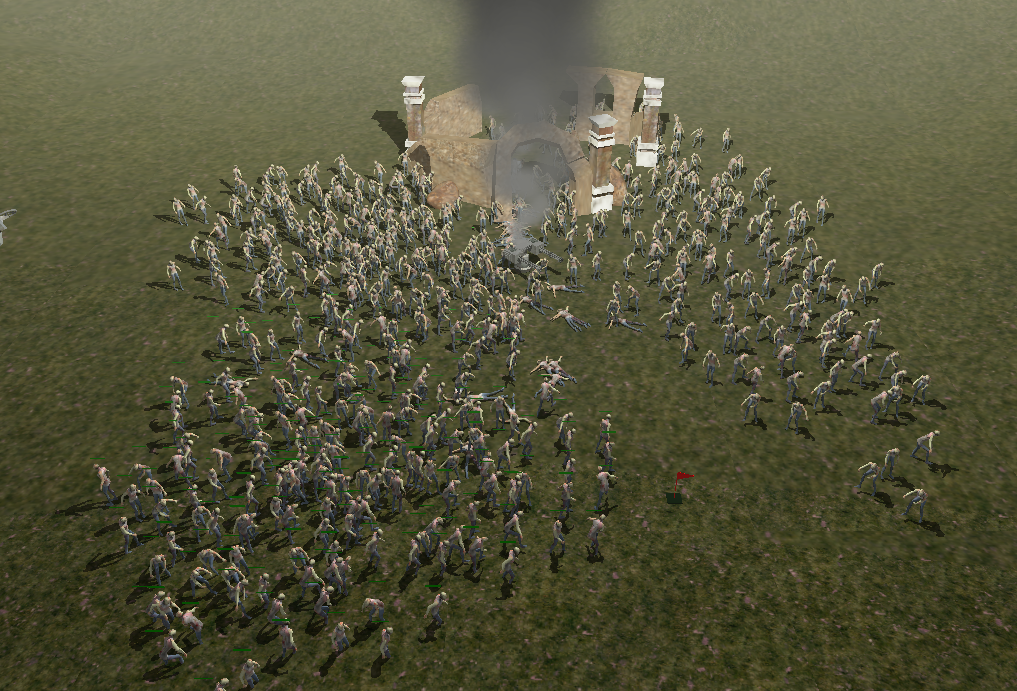
\includegraphics[scale=.6]{captura5.png}
	    \end{center}
	    \caption{Gameplay sample of the large number of units supported.}
	\end{figure}
	
\end{document}          
